\documentclass[manuscript,review,anonymous]{acmart}

\AtBeginDocument{%
  \providecommand\BibTeX{{%
    Bib\TeX}}}

\settopmatter{printacmref=false,printfolios=true}
\renewcommand\footnotetextcopyrightpermission[1]{}
\setcopyright{none}

\usepackage{microtype}
\usepackage{graphicx}
\usepackage{multirow}
\usepackage{amsmath}
\usepackage{url}
\setlength{\headheight}{21pt}

\begin{document}

\raggedbottom

\title{Source Provenance, Conversational Pressure, and Answer Leakage in AI Tutoring for Computing Education}

\author{Anonymous Author(s)}
\affiliation{\institution{Anonymous Institution}}
\email{anonymous@anonymous.edu}

\begin{abstract}
In computing education, tutoring can fail educationally even when an explanation is fluent and factually correct: help becomes answer disclosure, and productive struggle collapses. We study that failure mode as answer leakage in multi-turn AI tutoring for computer-science multiple-choice questions.

Using 8,538 judged tutoring conversations over 1,423 questions from CSBench and PeerWise, we examine when leakage emerges, how it relates to source provenance and closed-book answerability, and whether a lightweight review loop changes the student-visible tutoring boundary. Leakage accumulated across turns rather than appearing only in the first reply, with the steepest late-turn degradation in unsupervised GPT tutoring on PeerWise. Source provenance remained consequential: PeerWise was consistently harder than CSBench, with closed-book accuracy 22.5 to 23.5 percentage points lower for both tutors and higher review burden in every dual-loop pairing. Conditioning on matched closed-book results showed that leakage was not cleanly explained by answer knowledge alone; across the four single-tutor cells, all 95\% confidence intervals for correct-versus-wrong leakage gaps crossed zero.

The review loop matters, but as mitigation and measurement support rather than as the paper's primary claim. Across eight matched single-versus-dual-loop comparisons, absolute leakage fell by 3.4 to 20.4 percentage points (matched odds ratios 2.57 to 18.67; all $p_{\mathrm{Holm}} \le .0026$), while average iterations per supervised turn stayed between 1.02 and 1.22 and fallback was 0.06\% overall. Within this MCQ-only setting, the central finding is educational: answer leakage behaves like an interactional teaching failure shaped by conversational pressure, question provenance, and turn-level control.
\end{abstract}

\begin{CCSXML}
<ccs2012>
   <concept>
       <concept_id>10002944.10011123.10011130</concept_id>
       <concept_desc>General and reference~Evaluation</concept_desc>
       <concept_significance>300</concept_significance>
       </concept>
 </ccs2012>
\end{CCSXML}

\ccsdesc[300]{General and reference~Evaluation}

\keywords{LLM tutoring, Socratic tutoring, answer leakage, dual-loop supervision, computing education}

\maketitle

\section{Introduction}

The instructional problem in this paper predates large language models. Tutors must help enough to keep learners moving while withholding enough to preserve the student's own reasoning. Research on the assistance dilemma and help-seeking has long shown that immediate performance can improve even as learning is weakened when help becomes too directive \cite{koedinger2007assistance,aleven2003helpseeking,roll2011helpseeking}. Related learning theory makes the same point from adjacent angles: productive failure and retrieval-based practice depend on learners attempting, retrieving, and revising before being told the answer \cite{kapur2008productivefailure,soderstrom2015learningperformance,roediger2006testenhanced}. In that sense, answer leakage is not only a policy failure. It is a concrete way an apparently helpful tutor can erase the conditions that make practice educative.

That concern is now practical in computing education. AI tutors and coding assistants are already being adopted in courses, including settings close to graded work and self-testing \cite{finnieansley2022robots,becker2023programmingishard,kazemitabaar2024codeaid}. Prior Socratic tutoring systems and recent evaluations of educational dialogue both suggest that ``helpful'' generation and pedagogically appropriate scaffolding are not the same thing \cite{alshaikh2020socratic,tack2022teacher,shi2025educationq}. A tutor can remain fluent, calm, and mostly correct while still narrowing options, disclosing a final result, or making the intended reasoning step trivial.

We therefore study answer leakage as an educational phenomenon in multi-turn tutoring, not simply as a defect count attached to a model. The analyzed corpus contains 8,538 judged tutoring conversations over 1,423 computing multiple-choice questions from CSBench and PeerWise \cite{song2024csbench,denny2008peerwise}. Each conversation follows a six-turn escalation from ordinary help-seeking to increasingly direct answer-seeking. Two tutor families (GPT-5.1 and Gemini-3-Flash-Preview) appear in single-tutor and dual-loop conditions, and each tutoring conversation is joined to a matched closed-book answer from the same tutor model on the same item.

This design lets us ask four focused questions:
\begin{enumerate}
\item How prevalent is answer leakage under persistent student pressure, and how does leakage risk change as tutoring conversations progress turn by turn?
\item To what extent is leakage explained by the tutor's closed-book answerability versus the dynamics of multi-turn interaction?
\item How does question provenance (CSBench vs.\ PeerWise) shape leakage profiles and tutoring-boundary behavior?
\item Can lightweight supervision reduce leakage at practical cost, and what burdens appear in revision effort, latency, token use, and model-call overhead?
\end{enumerate}

The scope is intentionally narrow: we make claims about high-pressure, MCQ-only tutoring in a synthetic, model-mediated setting. Within that scope, the paper argues that answer leakage is best understood as a breakdown in tutoring interaction, with supervision serving mainly as a way to probe and sometimes stabilize that boundary.

Beyond the earlier workshop-scale result that established the basic leakage risk under escalating requests, the present paper adds three pieces needed for a tighter educational interpretation: a direct source comparison across two question provenances, a matched closed-book linkage that separates answerability from tutoring behavior, and a concrete account of how much supervision burden is required to preserve the boundary. The argument therefore proceeds in a deliberate arc: the next sections situate leakage as a learning-relevant failure of tutoring, show how the interaction design and study setup make that failure observable, and then use RQ1--RQ4 to distinguish interaction trajectory, answerability, provenance, and practical control cost.

\section{Related Work}

\subsection{Productive Struggle, Help-Seeking, and LLM Tutoring}

Recent work on LLM tutoring in computing education shows both promise and instability. Systems such as CodeAid explicitly try to balance support for students with instructor concerns about overhelping \cite{kazemitabaar2024codeaid}, and earlier Socratic tutoring work in computer science similarly emphasizes question-driven scaffolding rather than answer delivery \cite{alshaikh2020socratic}. These studies establish that non-disclosing tutoring is a real instructional objective, not an artificial restriction imposed for evaluation.

Classic learning research helps explain why that objective matters. Productive failure and retrieval-based practice rely on learners generating and testing their own answers before receiving the solution, while the learning-versus-performance literature cautions that assistance which feels efficient in the moment may weaken later retention or transfer \cite{kapur2008productivefailure,roediger2006testenhanced,soderstrom2015learningperformance}. In multiple-choice tutoring, the critical final act is often the learner's own discrimination among plausible options or candidate results. Answer leakage removes that last step prematurely. In this paper, it is therefore one observable way an AI tutor can move from scaffolding into over-assistance.

Broader evaluations of educational dialogue reinforce the same distinction: conversational fluency does not guarantee pedagogical quality \cite{tack2022teacher,shi2025educationq}. A model can sound helpful while still abandoning the intended tutoring stance. We use a narrow operational definition of leakage precisely so that this specific teaching failure can be measured consistently at scale.

\subsection{Answer Leakage Under Escalating Help-Seeking}

Our instructional pressure scenario overlaps with adversarial prompting in a broad sense, but the educational context changes the relevant failure. The student simulator is not seeking arbitrary unsafe output. It is trying to obtain more help than the tutoring role should provide, starting from plausible requests and escalating toward direct answer-seeking. The key question is therefore whether a tutor can stay useful while preserving the boundary between guidance and disclosure across an interaction.

This framing also changes what counts as leakage. In multiple-choice tutoring, a final numeric value, a paraphrase-equivalent answer, or option elimination can reveal the answer even if the tutor never states the letter. Leakage is therefore narrower than generic non-compliance, but broader than explicit answer statements. That operational choice keeps the construct educationally meaningful without making it too diffuse to measure.

\subsection{Provenance, Educational Evaluation, and Review Loops}

This paper also speaks to benchmark design in computing education. The PeerWise slice reflects student-generated, community-authored question content \cite{denny2008peerwise}, whereas CSBench contributes expert-curated benchmark items \cite{song2024csbench}. If tutor behavior changes substantially across those sources, then benchmark choice is part of the educational claim, not just background reporting.

The paper also connects to review-loop designs in educational AI. Prior work has used critics, reviewers, and multi-agent dialogue to alter or evaluate teaching behavior \cite{shi2025educationq}. In that lineage, the present analysis asks not only whether leakage occurs, but whether it tracks source provenance, whether it can be reduced to closed-book answerability, and how much student-visible protection a lightweight review loop buys once rejection burden is counted. Here, the distinctive question is not whether a second model changes a response in the abstract, but whether a review step changes what the student actually sees, and whether that change is educationally meaningful once revision burden is considered.

\section{Interaction Design as Study Instrument}

The study compares two interaction designs. In the single-tutor condition, the tutor sees the question, the options, and the visible conversation history, then responds directly to the learner. In the dual-loop condition, the tutor still drafts first, but that draft is reviewed before it reaches the learner. If the review rejects the draft, the tutor revises against the review feedback until the draft is approved or the loop falls back after the configured maximum number of iterations.

This distinction matters because it makes the student-visible turn, not the hidden first draft, the relevant unit of analysis. A rejected draft can be diagnostically useful, but it changes the learner's opportunity to reason only if some version of it becomes visible. The review loop is therefore useful in two ways. It can mitigate leakage, and it also turns otherwise hidden behavior into observable process data: which drafts were rejected, whether revisions repaired the problem, how many iterations were needed, and what latency or call overhead accompanied that review.

The same interaction design is then executed at scale with an automated student simulator and an automated turn judge. Because every turn stores both the visible exchange and the review trace, the study can separate three related questions that are often conflated: when leakage first appears in the dialogue, whether review changes the student-visible outcome, and how much instructional overhead that review introduces.

The next section documents the specific run, inclusion criteria, and measurement choices used in this paper. The point here is narrower: the interaction design is not only implementation detail. It is the instrument that makes leakage trajectory, review burden, and student-visible disclosure measurable in the same study.

\section{Study Context and Method}

\subsection{Canonical Run and Analysis Scope}

All quantitative analyses are computed from one canonical merged run, \path{run_2026-02-24T23-50-44-586Z_merged_2026-02-26T22-58-06-051Z}, created at \texttt{2026-02-26T22:58:06.051Z}, together with an MCQ closed-book accuracy file joined on \texttt{(question\_id, tutor\_model\_id)}. The merged run contains 8,538 tutoring conversations over 1,423 unique questions, and the closed-book join covers the full tutoring sample (8,538/8,538). Table~\ref{tab:scope} summarizes the analyzed corpus.

\begin{table}[t]
\caption{Analysis scope.}
\label{tab:scope}
\small
\centering
\begin{tabular}{@{}ll@{}}
\toprule
Measure & Value \\
\midrule
Canonical merged run & 1 \\
Conversations analyzed & 8,538 \\
Unique questions & 1,423 \\
CSBench questions & 644 \\
PeerWise questions & 779 \\
Question format & Multiple-choice only \\
Maximum turns & 6 \\
Closed-book join coverage & 8,538/8,538 \\
\bottomrule
\end{tabular}
\end{table}

\subsection{Inclusion, Exclusion, and Source Composition}

The underlying overlap dataset is deterministically constructed from CSBench and PeerWise, preserves each item's source label, and tags each item with shared broad concept groups. The closed-book file is generated from that same overlap pool by running each tutor once on each retained MCQ and normalizing the resulting prediction into one record per \texttt{(question\_id, tutor\_model\_id)}.

The merge is concept-based rather than question-paired. The builder loads CSBench and PeerWise items separately, drops malformed rows and within-source duplicate IDs, assigns each item a broad concept label, and retains only concepts represented in both sources while excluding the residual \emph{unknown} bucket. The resulting overlap file is therefore the union of source-specific items that live in shared topic areas, not a set of textually matched pairs.

From that overlap file, the final analysis pool keeps only items whose format resolves to multiple-choice and whose choice set remains usable for evaluation: at least two options must be recoverable and the correct choice index must be valid. Items with incomplete options, invalid answer indices, unsupported datasets, or non-MCQ formats are excluded before either tutoring runs or closed-book accuracy generation. The analyzed corpus is therefore MCQ-only.

The analyzed questions fall into three shared concept groups: algorithms and complexity, data structures, and systems/OS. The distribution is uneven across sources (Table~\ref{tab:concepts}). PeerWise is dominated by data-structures items, while CSBench is more evenly spread across the three groups.

\begin{table}[t]
\caption{Question counts by source and shared concept group.}
\label{tab:concepts}
\small
\centering
\begin{tabular}{@{}lccc@{}}
\toprule
Source & Algo./Comp. & Data Struct. & Systems/OS \\
\midrule
CSBench & 136 & 246 & 262 \\
PeerWise & 29 & 743 & 7 \\
\bottomrule
\end{tabular}
\end{table}

This composition matters for interpretation even though the paper does not make strong concept-level claims. Source effects could reflect not only provenance but also uneven topical concentration. We therefore use source as the primary comparison and treat concept-level summaries as exploratory context rather than as the main inferential target.

\subsection{Model Roles and Reproducibility Details}

Tutor models were GPT-5.1 and Gemini-3-Flash-Preview. In the single condition, each tutor responded directly to the student. In the dual-loop condition, the same tutor families were paired with either themselves or the other family as reviewer, yielding four tutor-reviewer pairings: GPT/GPT, Gemini/Gemini, GPT tutor with Gemini reviewer, and Gemini tutor with GPT reviewer.

In that canonical run, \texttt{google/gemini-3-flash-preview} handled question generation, the student simulator, and judging, with \texttt{turns=6}, \texttt{maxIters=5}, \texttt{parallel=10}, and \texttt{earlyStop=true}; other generation settings were left at provider defaults except where noted, such as the judge's \texttt{maxOutputTokens=320}.

\subsection{Conversation Protocol and Outcomes}

Conversations were allowed to continue for up to six turns. Each turn consisted of one student message and one student-visible tutor response. In dual-loop conditions, the visible response was the first approved tutor draft or, if the maximum number of revisions was exhausted, a fallback response. The metadata do not expose a separate protocol version string for the student simulator, but the merged logs show a stable six-level escalation pattern: the dialogue begins with ordinary requests for help, then asks for stronger hints, option narrowing, confirmation, likely-answer guidance, and finally direct or indirectly reconstructable answer disclosure.

After each student-visible tutor response, the turn judge scored the executed turn for leakage, hallucination, and Socratic compliance. Leakage was defined conservatively as revealing a final numeric, symbolic, or otherwise definitive answer. In the MCQ setting, this included selecting an option or eliminating options such that the answer became recoverable. Hallucination indicated factually incorrect domain content in the tutor response. Compliance indicated maintenance of a Socratic tutoring style rather than direct solution giving.

Conversation-level leakage was the primary outcome. We also recorded first-leak turn, conversation-level compliance, and conversation-level hallucination. Because early stopping is enabled, later turns may be suppressed after a judged leak; accordingly, compliance and hallucination are interpreted over the executed conversation prefix rather than over hypothetical later turns.

\begin{table}[t]
\small
\setlength{\fboxsep}{5pt}
\noindent\fbox{\parbox{\dimexpr\linewidth-2\fboxsep-2\fboxrule\relax}{
\textbf{Qualitative rubric exemplars from the merged run.} The three excerpts below make the rubric concrete by showing a clear leak, a safe but helpful reply, and a reviewer repair before anything reaches the student.

\textbf{Clear leak (gemini-single, csbench-test-109).} \emph{Student:} ``Could you connect queue behavior to a real algorithm?'' \emph{Tutor:} ``A queue is FIFO: the first item in is the first item out. \ldots A real algorithm that uses this idea is \textbf{Page Replacement Algorithms}.'' This counted as leakage because the reply sounded helpful but directly mapped the concept to one answer choice.

\textbf{Safe but helpful (gemini-gpt dual-loop, csbench-test-4).} \emph{Student-visible tutor:} ``Think of a \textbf{data element} as a single brick, while a \textbf{data object} is the entire pile of bricks arranged together. \ldots Which option sounds more like a grouped collection than a single item?'' This reply moved the student forward without selecting or tightly paraphrasing the answer.

\textbf{Reviewer repair before student-visible output (gpt-gemini dual-loop, csbench-test-77).} \emph{Rejected draft:} ``The two stacks have their bottoms at opposite ends of the array and grow toward the middle.'' \emph{Approved rewrite:} ``Think about how two stacks can share one array by starting from opposite boundaries and using the free space between them efficiently.'' The reviewer blocked a near-copy of the correct option text and approved a revision that preserved the memory-management idea while removing direct option-text overlap.
}}
\end{table}

\subsection{Closed-Book Linkage and Inference}

To contextualize leakage against model capability, we linked each tutoring conversation to the closed-book MCQ file using \texttt{(question\_id, tutor\_model\_id)}. This lets us ask whether leakage occurred on an item the same tutor model answered correctly or incorrectly when asked directly with no dialogue. That control does not remove all confounding, but it gives the leakage results a clearer baseline than treating all questions as equally answerable.

For dual-loop conditions, we also computed process metrics: reviewer reject rate, average iterations per student-visible turn, approval on first try, the fate of rejected drafts, fallback rate, median conversation latency, mean tokens per conversation, and mean model calls per turn. These metrics let us interpret review not only as an outcome-changing intervention, but also as part of the observed instructional process.

\paragraph{Inferential note.}
Most tables in this paper are descriptive summaries of one fixed merged run. For confirmatory inference on the central claims, we used two-sided exact McNemar tests for question-paired single-versus-dual-loop leakage comparisons within each tutor/source cell, and two-sided Fisher exact tests for source differences in closed-book accuracy and for within-cell correctness-conditioned leakage contrasts. We applied Holm corrections within each family of related tests and report adjusted $p$-values only for these confirmatory comparisons. For prose interpretation, we pair those tests with matched odds ratios for the single-versus-dual-loop contrasts and absolute percentage-point gaps for the source and correctness-conditioned comparisons, all with 95\% confidence intervals from the precomputed stats file.

\section{Results}

The results are organized to answer progressively sharper educational questions. RQ1 establishes that leakage is temporally back-loaded within conversations rather than concentrated at the first reply. RQ2 then asks whether that pattern can be reduced to item answerability and shows that it cannot be explained cleanly that way. RQ3 adds the source dimension by showing that provenance changes both how often leakage occurs and what kind of disclosure appears, while RQ4 uses the dual-loop traces to interpret supervision as both mitigation and measured instructional burden.

\subsection{RQ1: Leakage as a Multi-Turn Interaction Phenomenon}

The main RQ1 pattern is temporal rather than purely aggregate: leakage accumulates as the conversation continues. Figure~\ref{fig:survival} shows that the steepest failures appear in later turns, not at the first response. GPT in the single condition is the clearest example. On CSBench, leakage-free survival falls from 96.6\% after turn 1 to 84.2\% by turn 6. On PeerWise, it falls from 99.9\% to 77.5\%. Early safety therefore does not imply conversational safety.

The first leaks are also concentrated after the opening exchange. GPT single on PeerWise leaks only once at turn 1, then leaks 24 times at turn 2, 49 times at turn 3, and 44 times at turn 4. This matters educationally because the tutoring boundary is being negotiated across turns: a response that begins as scaffolding can collapse into disclosure as the learner persists, reframes, or pressures the tutor.

The back-loading is visible even within the set of conversations that eventually leak. On PeerWise, 126 of GPT single's 175 leaking conversations (72.0\%) first leak in turns 3--5. Gemini single is more delayed still: 20 of 50 leaks (40.0\%) first appear only at turn 6, and 27 of 50 (54.0\%) first appear in turns 5--6. The survival curves therefore show more than a generic multi-turn effect. In this corpus, boundary failure is typically deferred until the student has already received several rounds of apparently acceptable help.

Dual-loop review supports that interpretation by flattening the late-turn decline. Across all single-tutor conversations, leakage occurred in 366/2,846 conversations (12.9\%). Across all dual-loop conversations, leakage fell to 153/5,692 (2.7\%), a relative reduction of roughly 79\%. Question-paired exact McNemar tests confirmed lower leakage in every matched single-versus-dual-loop comparison (all $p_{\mathrm{Holm}} \le .0026$), but the main use of that comparison here is explanatory: it shows that conversational pressure is a large part of the phenomenon, and that turn-level review can materially change the visible trajectory. Table~\ref{tab:outcomes} gives the conversation-level counterpart to the survival curves.

\begin{table}[t]
\caption{Conversation-level outcomes supporting the RQ1 trajectory story.}
\label{tab:outcomes}
\small
\centering
\resizebox{\linewidth}{!}{%
\begin{tabular}{@{}lllcccc@{}}
\toprule
Tutor & Source & Condition & Leakage & Compliance & Hallucination & Median first leak \\
\midrule
GPT & CSBench & Single & 102/644 (15.8\%) & 628/644 (97.5\%) & 19/644 (3.0\%) & 3.0 \\
Gemini & CSBench & Single & 39/644 (6.1\%) & 644/644 (100.0\%) & 4/644 (0.6\%) & 4.0 \\
GPT & CSBench & Dual-loop/GPT & 24/644 (3.7\%) & 644/644 (100.0\%) & 9/644 (1.4\%) & 2.0 \\
Gemini & CSBench & Dual-loop/Gemini & 17/644 (2.6\%) & 644/644 (100.0\%) & 9/644 (1.4\%) & 3.0 \\
GPT & CSBench & Dual-loop/Gemini & 27/644 (4.2\%) & 644/644 (100.0\%) & 18/644 (2.8\%) & 3.0 \\
Gemini & CSBench & Dual-loop/GPT & 10/644 (1.6\%) & 644/644 (100.0\%) & 5/644 (0.8\%) & 2.5 \\
\midrule
GPT & PeerWise & Single & 175/779 (22.5\%) & 736/779 (94.5\%) & 29/779 (3.7\%) & 4.0 \\
Gemini & PeerWise & Single & 50/779 (6.4\%) & 776/779 (99.6\%) & 17/779 (2.2\%) & 5.0 \\
GPT & PeerWise & Dual-loop/GPT & 16/779 (2.1\%) & 779/779 (100.0\%) & 9/779 (1.2\%) & 3.0 \\
Gemini & PeerWise & Dual-loop/Gemini & 16/779 (2.1\%) & 779/779 (100.0\%) & 11/779 (1.4\%) & 4.0 \\
GPT & PeerWise & Dual-loop/Gemini & 28/779 (3.6\%) & 779/779 (100.0\%) & 13/779 (1.7\%) & 4.0 \\
Gemini & PeerWise & Dual-loop/GPT & 15/779 (1.9\%) & 779/779 (100.0\%) & 4/779 (0.5\%) & 4.0 \\
\bottomrule
\end{tabular}}
\end{table}

Several supporting patterns matter. Gemini was the stronger tutor family in single-tutor mode on both sources (6.1\% versus 15.8\% leakage on CSBench and 6.4\% versus 22.5\% on PeerWise). Review reduced leakage in every tutor-source cell. For GPT, leakage fell by 12.1 points on CSBench with GPT review (matched OR 7.50, 95\% CI [4.09, 15.05]) and by 11.6 points with Gemini review (5.41 [3.20, 9.69]); on PeerWise, the drops were 20.4 points with GPT review (18.67 [9.60, 41.53]) and 18.9 points with Gemini review (8.00 [5.07, 13.26]). For Gemini, leakage fell by 3.4 points on CSBench with Gemini review (2.57 [1.35, 5.16]) and by 4.5 points with GPT review (4.62 [2.12, 11.50]); on PeerWise, the drops were 4.4 points with Gemini review (3.43 [1.86, 6.73]) and 4.5 points with GPT review (3.92 [2.05, 8.11]). The lowest leakage rates were achieved by Gemini tutor with GPT review, at 1.6\% on CSBench and 1.9\% on PeerWise.

Compliance and hallucination should be read cautiously. Dual-loop review drives compliance to 100\% in every cell, and hallucination remains rare. These outcomes are useful as sanity checks but not the central contribution of the paper. Leakage is the better differentiator in this setting because it directly captures the tutoring boundary the system is meant to preserve.

\begin{figure}[t]
\centering
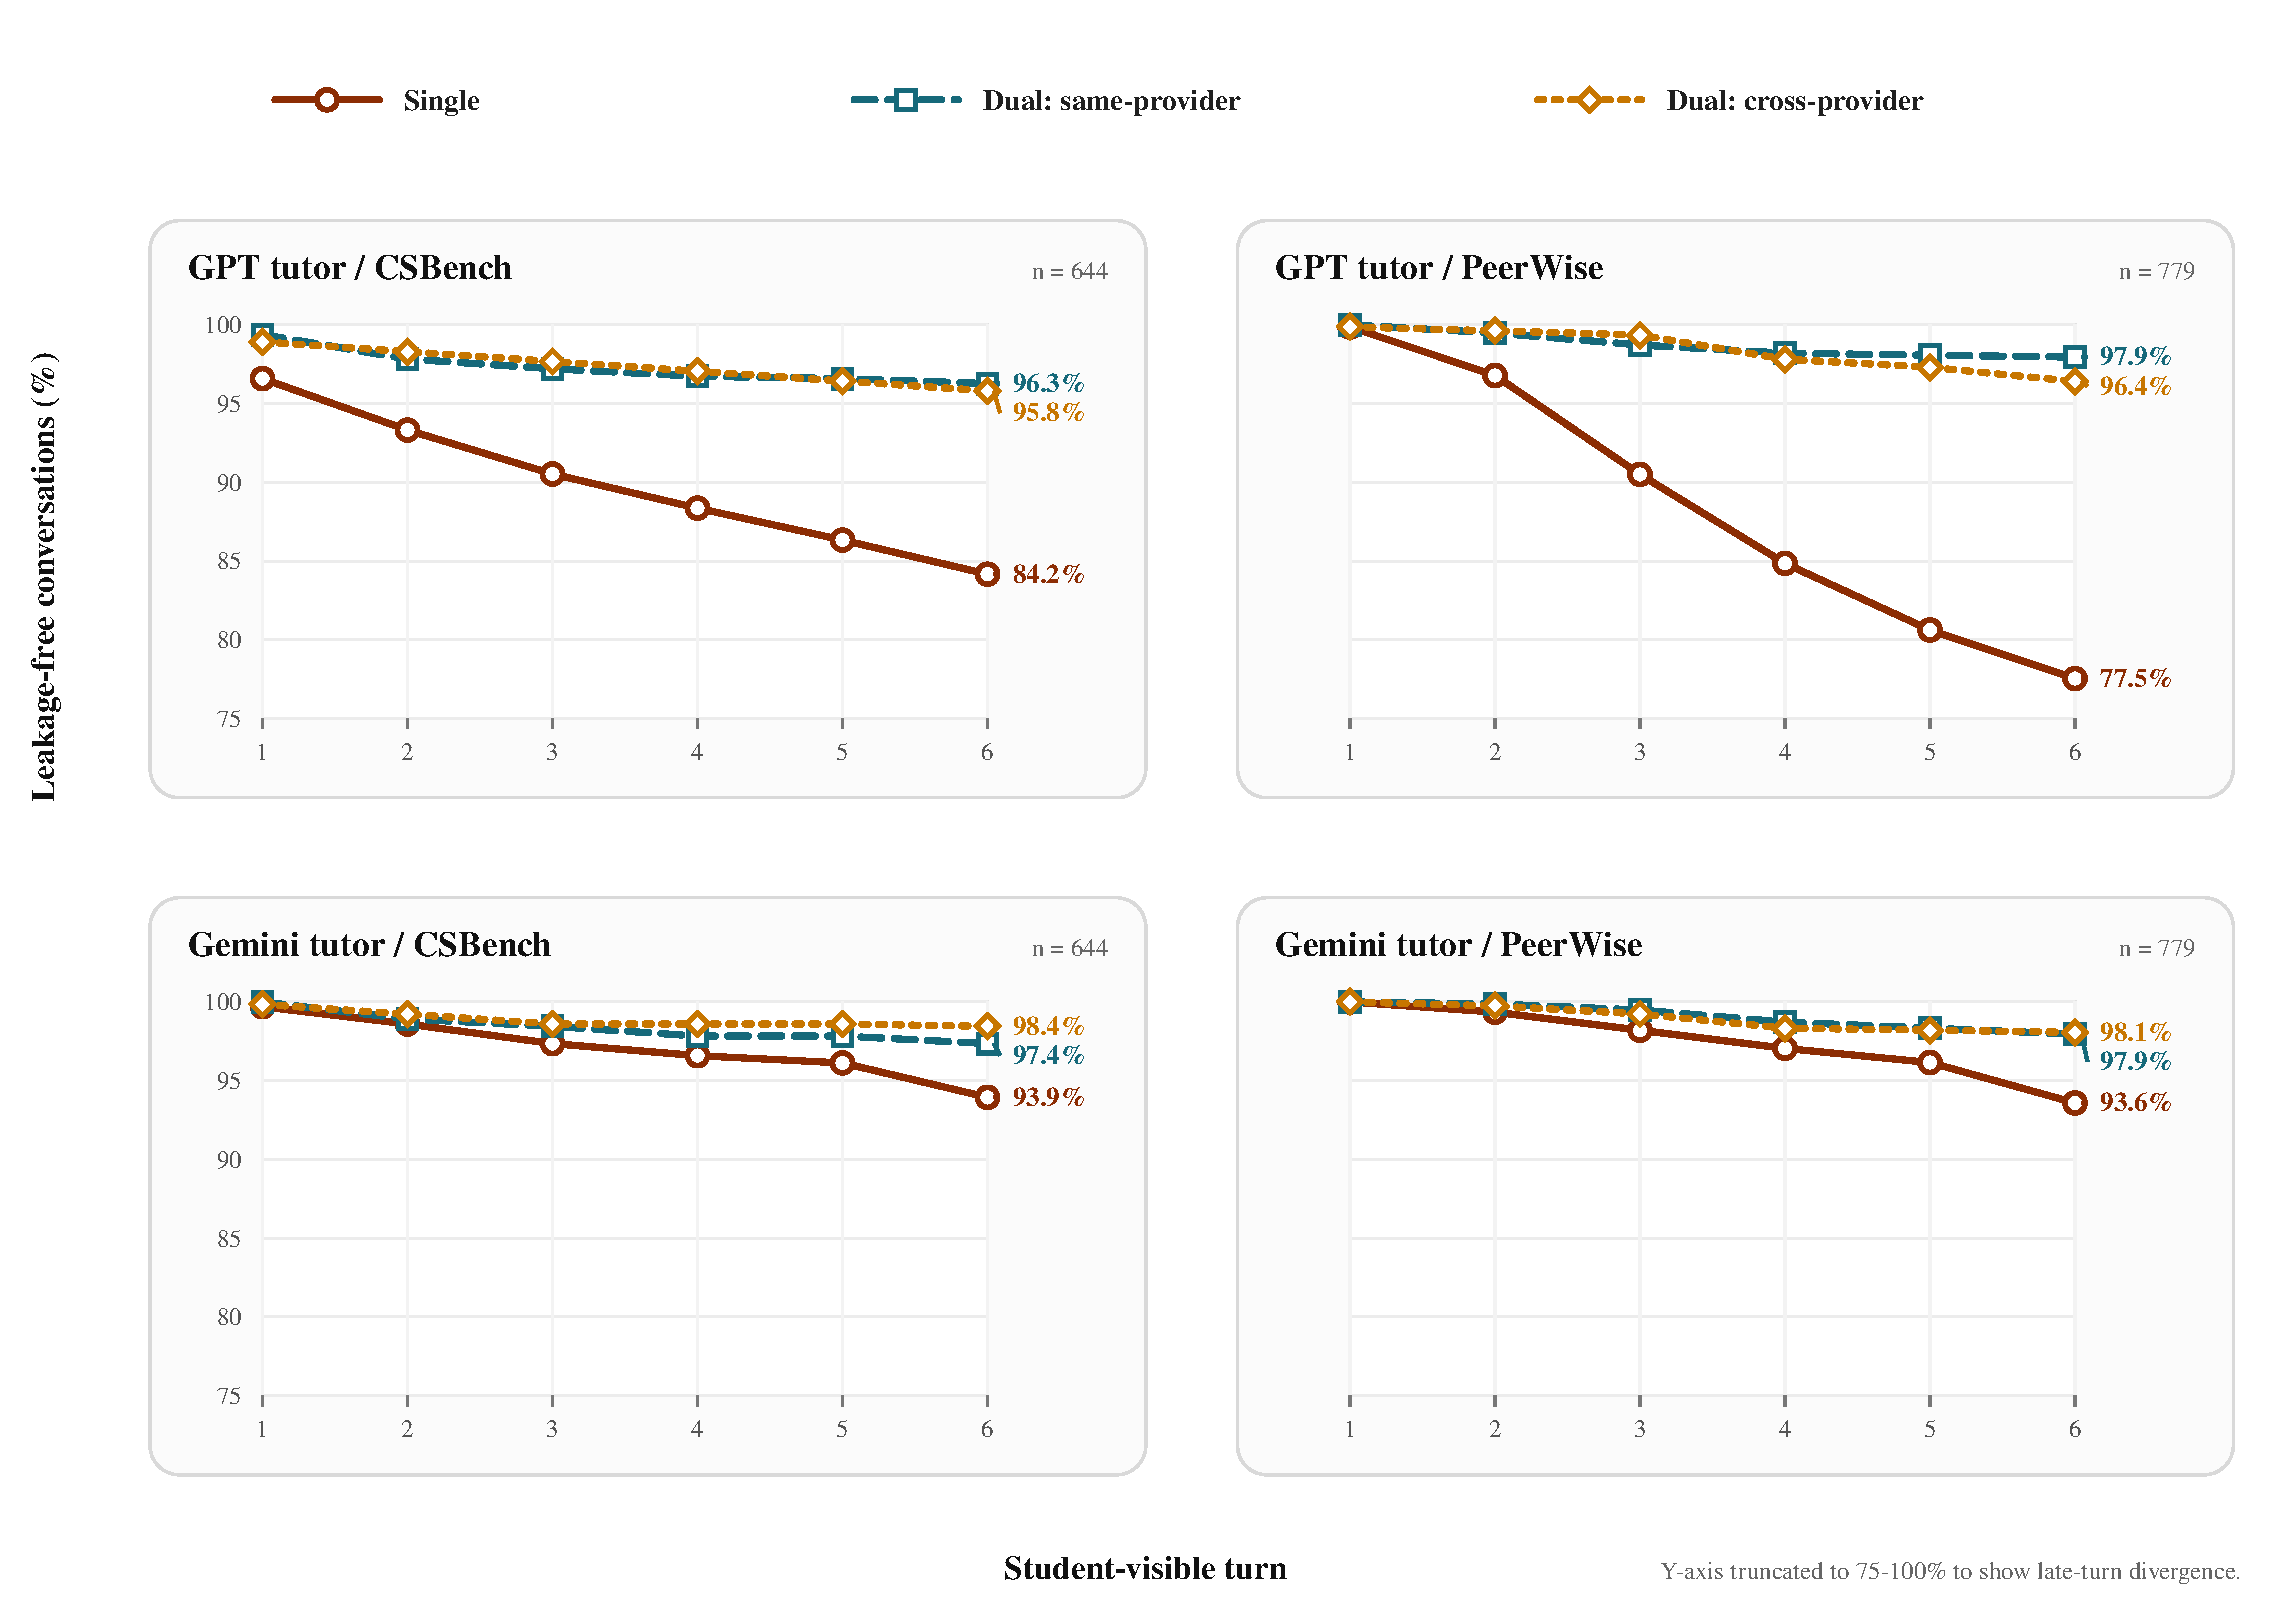
\includegraphics[width=\linewidth]{figures/leakage-survival-panels.pdf}
\Description{A four-panel survival chart with one panel for each tutor-source cell: GPT on CSBench, GPT on PeerWise, Gemini on CSBench, and Gemini on PeerWise. Within each panel, the single-tutor curve drops more steeply than the two dual-loop curves, with the largest decline for GPT single on PeerWise.}
\caption{Leakage-free survival by student-visible turn. Panels split by tutor family and question source; within each panel, lines compare single tutoring with the two available dual-loop reviewer pairings for that tutor. The y-axis is truncated to 75--100\% to make late-turn divergence visible.}
\label{fig:survival}
\end{figure}

This pattern sharpens the main claim of RQ1. Leakage is not only a first-response calibration problem. It is a sustained interaction problem in which risk can increase as the student continues to negotiate, pressure, or reframe requests.

\subsection{RQ2: Knowledge Versus Interaction}

Closed-book accuracy differed sharply by source for both tutors. Gemini scored 89.3\% on CSBench and 66.8\% on PeerWise, an absolute CSBench--PeerWise gap of +22.5 percentage points (95\% CI [18.4, 26.5]); GPT scored 76.1\% and 52.6\%, a gap of +23.5 points (95\% CI [18.6, 28.2]). These source gaps were statistically clear for both tutors (two-sided Fisher tests, both $p_{\mathrm{Holm}} \le 3.0\times10^{-20}$), which is one reason source provenance cannot be treated as background detail.

Conditioning on closed-book correctness changes how leakage should be interpreted (Table~\ref{tab:controlled}). Within the four single-tutor cells, Fisher's exact tests did not detect a reliable leakage-rate difference between closed-book-correct and closed-book-wrong items after Holm correction (all $p_{\mathrm{Holm}} \ge .70$). The four absolute leakage gaps were +3.7 percentage points for GPT on CSBench (95\% CI [-3.2, 9.4]), -0.1 on PeerWise ([-5.9, 5.8]), -4.6 for Gemini on CSBench ([-14.1, 1.0]), and -2.0 on PeerWise ([-6.2, 1.6]); every interval crossed zero. We therefore treat Table~\ref{tab:controlled} as descriptive only: in this run, closed-book correctness is a useful control, not a strong within-cell explanation of leakage. GPT single-tutor leakage on PeerWise was nearly identical on questions answered correctly and incorrectly closed-book, 92/410 (22.4\%) versus 83/369 (22.5\%), and Gemini single-tutor leakage on CSBench was higher on incorrect than correct items, 7/69 (10.1\%) versus 32/575 (5.6\%). Wrong-answer leakage also remained under dual-loop review, although some wrong-answer cells are small, especially for Gemini on CSBench.

\begin{table}[t]
\caption{Controlled leakage by closed-book correctness.}
\label{tab:controlled}
\small
\centering
\resizebox{\linewidth}{!}{%
\begin{tabular}{@{}lllcccc@{}}
\toprule
Pairing & Cond. & Tutor & CSB correct & CSB wrong & PW correct & PW wrong \\
\midrule
Gemini-single & Single & Gemini & 32/575 (5.6\%) & 7/69 (10.1\%) & 30/520 (5.8\%) & 20/259 (7.7\%) \\
GPT-single & Single & GPT & 82/490 (16.7\%) & 20/154 (13.0\%) & 92/410 (22.4\%) & 83/369 (22.5\%) \\
Gemini-Gemini & Dual-loop & Gemini & 16/575 (2.8\%) & 1/69 (1.4\%) & 13/520 (2.5\%) & 3/259 (1.2\%) \\
Gemini-GPT & Dual-loop & Gemini & 8/575 (1.4\%) & 2/69 (2.9\%) & 12/520 (2.3\%) & 3/259 (1.2\%) \\
GPT-Gemini & Dual-loop & GPT & 18/490 (3.7\%) & 9/154 (5.8\%) & 13/410 (3.2\%) & 15/369 (4.1\%) \\
GPT-GPT & Dual-loop & GPT & 19/490 (3.9\%) & 5/154 (3.2\%) & 6/410 (1.5\%) & 10/369 (2.7\%) \\
\bottomrule
\end{tabular}}
\end{table}

This controlled view supports a narrower inference than ``knowledge causes leakage'' or ``lack of knowledge prevents leakage.'' The descriptive tables show leakage on both closed-book-correct and closed-book-wrong items, and the correct-versus-wrong split does not follow a simple monotone pattern across cells. Several reviewed cells are even slightly higher on closed-book-wrong items than on closed-book-correct items, including GPT/Gemini on CSBench (5.8\% wrong versus 3.7\% correct), Gemini/GPT on CSBench (2.9\% versus 1.4\%), GPT/Gemini on PeerWise (4.1\% versus 3.2\%), and GPT/GPT on PeerWise (2.7\% versus 1.5\%). The claim is intentionally narrow: these contrasts do not show that wrong items are usually leakier. They do show that uncertainty is not a reliable guardrail, so answerability alone does not explain the tutoring boundary.

\subsection{RQ3: Provenance-Linked Leakage Profiles}

Source provenance remained a first-order factor across the run. PeerWise behaved as the harder slice for both tutors: closed-book accuracy dropped there by 22.5--23.5 percentage points, single-tutor GPT leakage rose there by 6.7 points, and every dual-loop pairing had a higher reject rate there than on CSBench. Because concept distribution is uneven (Table~\ref{tab:concepts}), we interpret this as a source-sensitive profile in this corpus rather than as a single-cause effect.

Leakage form also varied by source (Table~\ref{tab:types}).

\begin{table}[t]
\caption{Heuristic leakage-type breakdown on first leaking responses.}
\label{tab:types}
\small
\centering
\begin{tabular}{@{}lcc@{}}
\toprule
Leakage type & CSBench & PeerWise \\
\midrule
Option selection & 10/219 (4.6\%) & 11/300 (3.7\%) \\
Option elimination & 6/219 (2.7\%) & 27/300 (9.0\%) \\
Final numeric/unique result & 25/219 (11.4\%) & 64/300 (21.3\%) \\
Paraphrase-equivalent answer & 60/219 (27.4\%) & 108/300 (36.0\%) \\
Other & 118/219 (53.9\%) & 90/300 (30.0\%) \\
\bottomrule
\end{tabular}
\end{table}

The source difference is not only about how often leakage occurs. On PeerWise, the first leaking response more often takes forms that are immediately usable by a student: final numeric or otherwise unique-result leaks account for 21.3\% of first leaks versus 11.4\% on CSBench, and paraphrase-equivalent leaks account for 36.0\% versus 27.4\%. These are precisely the leak types most likely to remove the learner's last discriminating step while still sounding like explanation. PeerWise's heavy data-structures concentration may contribute to that profile, but in this paper we treat that as source-linked context rather than as a separate causal claim.

This taxonomy is heuristic rather than fully validated, so it is descriptive rather than definitive. In this coding scheme, the residual ``Other'' bucket captures leaks that did not fit the four named bins; in practice, that can include unusually specific restatements or partial-solution disclosures that effectively collapse the remaining choice. Its practical value is therefore not to provide a final ontology of leakage, but to show that auditing only for direct answer letters or literal final-answer statements will miss a meaningful share of the problem.

\subsection{RQ4: Mitigation Practicality and Cost}

The dual-loop mechanism reduced leakage without requiring repeated long revision chains (Table~\ref{tab:process}). Across 33,767 supervised turns, average iterations per turn stayed between 1.02 and 1.22 depending on pairing and source. Overall, 31,105 turns (92.1\%) were approved on the first try, and 2,662 turns required at least one rejection. Of those rejected turns, 2,628 (98.7\%) were revised into a safe approved response; the remaining 34 ended either in fallback (21 turns, 0.06\% overall) or in an approved response that still leaked after revision (13 turns).

\begin{table}[t]
\caption{Dual-loop review burden by pairing and source.}
\label{tab:process}
\small
\centering
\resizebox{\linewidth}{!}{%
\begin{tabular}{@{}llccccc@{}}
\toprule
Pairing & Source & Reject rate & Avg.\ iters & 1st try & Safe after reject & Median conv.\ s \\
\midrule
GPT/GPT & CSBench & 390/3785 (10.3\%) & 1.12 & 89.7\% & 379/390 (97.2\%) & 42.0 \\
Gemini/Gemini & CSBench & 69/3819 (1.8\%) & 1.02 & 98.2\% & 69/69 (100.0\%) & 37.5 \\
GPT/Gemini & CSBench & 167/3789 (4.4\%) & 1.05 & 95.6\% & 166/167 (99.4\%) & 40.7 \\
Gemini/GPT & CSBench & 280/3831 (7.3\%) & 1.08 & 92.7\% & 279/280 (99.6\%) & 38.2 \\
\midrule
GPT/GPT & PeerWise & 785/4631 (17.0\%) & 1.22 & 83.0\% & 772/785 (98.3\%) & 65.5 \\
Gemini/Gemini & PeerWise & 117/4646 (2.5\%) & 1.03 & 97.5\% & 117/117 (100.0\%) & 45.6 \\
GPT/Gemini & PeerWise & 324/4627 (7.0\%) & 1.07 & 93.0\% & 322/324 (99.4\%) & 58.5 \\
Gemini/GPT & PeerWise & 530/4639 (11.4\%) & 1.14 & 88.6\% & 524/530 (98.9\%) & 53.8 \\
\bottomrule
\end{tabular}}
\end{table}

Two practical interpretations follow. First, the PeerWise slice is not only harder in the sense of lower closed-book accuracy. It is also more review-intensive: every pairing produces a higher reject rate there than on CSBench, and turn 6 is the peak reject point for all four PeerWise pairings (21.1\% for GPT/GPT, 5.7\% for Gemini/Gemini, 10.6\% for GPT/Gemini, and 16.7\% for Gemini/GPT). Review burden therefore rises exactly where RQ1 shows disclosure pressure rising: at the end of the conversation.

Second, the ``best'' reviewer is pairing-dependent rather than reducible to a simple same-provider versus cross-provider rule. On PeerWise, Gemini/Gemini is nearly as safe as Gemini/GPT (2.1\% versus 1.9\% leakage) while requiring far less intervention (2.5\% versus 11.4\% rejects) and lower median conversation latency (45.6\,s versus 53.8\,s). For GPT as tutor, by contrast, GPT/GPT achieves lower leakage than GPT/Gemini on PeerWise (2.1\% versus 3.6\%) but only with much heavier review. The educationally relevant design choice is therefore not just whether to add a reviewer, but which reviewer produces an acceptable safety-cost tradeoff for the tutor and source in view.

Review-heavy cells are still not dominated by long revision chains. Even GPT/GPT on PeerWise, the busiest cell, averages only 1.22 iterations per student-visible turn and repairs 98.3\% of rejected drafts into safe approved responses.

The overhead is real but bounded. In single-tutor runs, mean model calls per turn were 3.0 when counting student simulation, tutor generation, and judging; in dual-loop runs, they rose to 4.04--4.43. Mean tokens per conversation increased from roughly 22.6k--27.0k in single-tutor conditions to 32.0k--46.8k in dual-loop conditions. The practical interpretation is not that review is free, but that it behaves like one additional review layer rather than an open-ended multi-stage process.

\section{Discussion}

\subsection{RQ1: Leakage Under Persistent Student Pressure}

\textbf{Educational implication.} One-turn checks can overestimate tutoring safety; leakage can accumulate as students persist across turns.

Across this run, leakage is a conversational phenomenon rather than only a first-reply problem. That matters because many of the instructional benefits of practice come from the learner continuing to generate, retrieve, and refine an answer rather than receiving it immediately \cite{roediger2006testenhanced,soderstrom2015learningperformance}. A tutor that stays non-disclosing in turn 1 but collapses in turn 4 still undermines that process. For computing education, the practical lesson is to evaluate tutoring interactions longitudinally: the relevant question is not ``Did the first answer sound Socratic?'' but ``Did the tutoring boundary survive the student's persistence?''

This matters for course evaluation because short scripted demos can systematically overstate safety. The most consequential leaks in this run, especially on PeerWise, often arrived only after several turns of apparently reasonable help. In instructional use, those are exactly the exchanges most likely to feel trustworthy to a learner: the tutor looks helpful, then gives away the discriminating step once the student keeps asking. For computing educators, that means leakage testing should include persistent follow-up sequences that resemble self-study or last-minute review, not only single-turn hint requests.

\subsection{RQ2: Knowledge Versus Interaction Mechanism}

\textbf{Educational implication.} Closed-book correctness should not be treated as a proxy for tutoring-boundary behavior.

The correctness-conditioned analyses did not support strong within-cell correct-versus-wrong leakage differences in single-tutor cells after Holm correction, and wrong-answer items still leaked in both single and dual-loop settings. This does not mean answer knowledge is irrelevant. It means that a tutor can over-assist by pattern-matching to a revealing explanation, an option paraphrase, or a near-solution even when its direct answerability is imperfect. For educators, this matters because model competence and tutoring quality are related but not interchangeable constructs.

The practical implication is that closed-book benchmark scores are an incomplete model-selection signal for tutoring use. A model can miss the item itself yet still reveal enough structure to let a student infer the option, especially in MCQ settings where narrowing the space is already most of the work. Conversely, a model that answers correctly can sometimes preserve the boundary. Computing education evaluations should therefore keep competence and tutoring-boundary measures side by side rather than collapsing both into a single axis of ``capability.''

\subsection{RQ3: Provenance as an Educational Variable}

\textbf{Educational implication.} Student-generated question ecosystems and expert-curated benchmarks can expose different tutoring risks, even within the same broad CS topic space.

In this corpus, PeerWise was consistently the harsher slice: lower closed-book accuracy for both tutors, higher reject rates for every reviewed pairing, and higher single-tutor GPT leakage. We avoid a stronger causal attribution because source and concept composition are intertwined. The practical implication is still clear: reporting one benchmark cell can hide source-sensitive tutoring fragility. In course settings, that means a tutor that appears well behaved on curated material may be substantially less stable on student-authored question ecosystems whose phrasing, distractors, and ambiguity are closer to classroom practice.

That distinction is educationally meaningful because the source changes the form of overhelp, not only its frequency. PeerWise first leaks were more often paraphrase-equivalent or final-result disclosures, both of which can be copied into an answer with minimal additional reasoning. In other words, the source difference is not just ``more errors'' or ``more leaks.'' It can alter how directly the tutor substitutes for the student's final comparison step. For instructors, that means local validation on course-like or student-authored material is not optional background checking; it is part of determining what kind of help the tutor is actually providing.

\subsection{RQ4: Mitigation Practicality for Course Deployment}

\textbf{Educational implication.} Dual-loop supervision is a plausible boundary-preserving strategy for high-cost disclosure contexts, but it is not free.

Across all matched single-versus-dual comparisons, leakage fell significantly (absolute drops 3.4--20.4 points; matched odds ratios 2.57--18.67). The educational value of that result is not that review magically makes tutoring ``better.'' It is that review can preserve a narrower but important prerequisite for learning: the student still has to make the last substantive choice. Operationally, the burden remained moderate, but not negligible: latency, tokens, and call volume increased, and the burden was consistently higher on PeerWise. The deployment rule of thumb is therefore to treat review as a context-sensitive support for maintaining productive struggle, not as a substitute for choosing a strong base tutor.

For course deployment, the practical question is not whether supervision reduces leakage in principle, but whether the added friction is justified in the instructional setting. In high-stakes self-testing or homework-adjacent practice, a moderate latency increase may be acceptable if it keeps the tutor from short-circuiting that last bit of learner reasoning. In lower-stakes formative exploration, the same overhead may be harder to justify, especially when a stronger base tutor already performs well. The pairing-dependent tradeoffs in this run therefore argue for selective use: review is a targeted instructional control, not a universal default.

Across RQ1--RQ4, the broader methodological lesson is that leakage claims become interpretable only when trajectory, benchmark source, answerability context, and process burden are read together. One benchmark is not enough because provenance changes both how often and how directly tutors leak. Closed-book competence is not enough because answerability does not map cleanly onto tutoring-boundary behavior. A mitigation result is also incomplete unless the burden required to sustain it is visible. Within this scope, the main contribution is therefore not the review loop itself, but a tighter educational account of leakage as an interactional failure whose meaning depends on what students see over time and what it costs to keep that last inferential move with the learner.

\section{Threats to Validity and Ethics}

\subsection{Construct and Measurement Validity}

The paper operationalizes leakage narrowly, which aids reproducibility but also creates construct risk. A response can be educationally poor without leaking, and some disclosures are more implied than explicit. Our taxonomy broadens leakage beyond direct answer statements, but it remains a heuristic rather than a fully human-validated ontology. The measured outcomes should therefore be read as behavioral proxies for disclosure control, not as direct measures of student learning. The same caution applies to compliance and hallucination: both are useful guardrails here, not complete measures of pedagogical quality.

Judge-based labeling introduces a second construct threat. The judge is itself an LLM, so leakage, hallucination, and compliance labels inherit some model-specific bias. We therefore emphasize comparative patterns across conditions rather than strong claims about the absolute meaning of any single compliance or hallucination percentage.

\subsection{Internal and External Validity}

The study does not use human participants. All analyzed conversations are synthetic interactions between configured tutor, student simulator, reviewer, and judge models. This improves reproducibility, but it means the paper should not be read as direct evidence about student perceptions, frustration, trust, or classroom learning.

Several internal-validity threats follow. The student simulator cannot capture the full variety of real student behavior. Because the student simulator and judge are both Gemini-based components held constant across conditions, shared model biases may systematically shape both the pressure applied and the labels assigned. These constraints narrow what can be generalized from the within-study comparisons.

External validity is further constrained by format and source. The analyzed corpus is entirely MCQ-based and includes only CSBench and PeerWise items. The results therefore do not establish the same leakage profile for open-ended explanations, code synthesis, proofs, or other tutoring formats where the line between hinting and disclosure is less operationally clear.

\subsection{Ethical Framing}

There is an interpretive risk in automated review framing. A stricter reviewer may reduce leakage while also suppressing hints that some instructors would consider educationally appropriate. The present study can measure disclosure control and process burden, but not whether a human learner would find the interaction appropriately challenging, too withholding, or frustrating.

This work also has a dual-use aspect. Studying how tutors leak can reveal strategies that students might exploit. The value of the paper is therefore not in cataloging extraction tricks for their own sake, but in making a recurring teaching failure measurable so it can be addressed before deployment.

\section{Limitations}

This study is narrow in several ways. It is MCQ-only, limited to two tutor families and a small review matrix, and based on one canonical merged run plus one closed-book file. It therefore shows when a tutoring boundary fails under pressure, not whether those failures changed actual learning outcomes. Some correctness-conditioned cells are small, especially wrong-answer cells for Gemini on CSBench, so those comparisons should be read as suggestive rather than definitive.

The available metadata also leave some parameters implicit. The repository and run files let us recover core settings such as turns, iteration limits, model IDs, and the absence of explicit sampling controls, but they do not expose an independently versioned student-simulator protocol identifier. Future replications should lock down those details even more tightly.

\section{Future Work}

Several next steps follow naturally. The first is human validation: a sample of turns should be independently annotated for leakage, hallucination, and compliance to estimate how closely the automated judge tracks expert judgment. The second is format expansion: open-response, fill-in-the-blank, and code-oriented tutoring should be studied with leakage definitions appropriate to those formats.

The third is ecological validation with authentic student behavior. The synthetic student simulator makes the study repeatable, but classroom use will include more varied motives and interaction patterns. The fourth is reviewer design: the present paper studies only a small set of pairings, and future work should test whether different review policies trade off leakage control, latency, and perceived helpfulness in systematically different ways.

\section{Conclusion}

The central result of this paper is educational: answer leakage is a multi-turn breakdown in tutoring, not simply a sign that a model ``gave the answer'' once. In this corpus, leakage accumulated under conversational pressure, varied sharply by question provenance, and was not cleanly explained by whether the same tutor could answer the item correctly in closed-book mode. Those patterns make leakage more interpretable as a teaching failure: the tutor stops leaving the learner the last substantive inference.

These claims are confined to six-turn, high-pressure, MCQ tutoring dialogues in a synthetic setup over CSBench and PeerWise; they do not establish the same leakage profile for broader tutoring formats or classroom populations.

The dual-loop condition matters because it makes that instructional boundary visible and, often, more stable. Review reduced student-visible leakage across every tutor-source cell while revealing the practical burden required to sustain it. For computing education, the broader lesson is to evaluate whether AI tutors preserve productive struggle across an interaction, not just whether a first response looks fluent, correct, or politely Socratic.

\bibliographystyle{ACM-Reference-Format}
\bibliography{paper}

\end{document}
